\section{Randomized Selection}
\subsection{Algoritme}
Tager en uordnet liste $S$ med $n$ elementer og $k \in \{1, ..., n\}$ som input og returnerer det $k$'te mindste element i $S$.\\

I følgende bruger vi notationen:\\
$L_{(i)}$: Det $i$'te mindste element i en liste $L$.\\
$r_L(a)$: Rank af element $a$ i listen $L$.\\


\texttt{LazySelect}$(S, k)$
\begin{enumerate}
  \item Vælg $n^{3/4}$ elementer uafhængigt og uniformt tilfældigt fra $S$. Lad $R$ være en multimængde af valgte elementer.
  \item Sorter $R$ (dette ødelægger ikke vores køretid da $R$ relativt set er lille).
  \item Lad $x = kn^{-1/4}$ og
  \begin{align*}
    l = \max\{\floor{x - \sqrt{n}}, 1\}
    \quad\quad & \quad\quad
    h = \min\{\ceil{x + \sqrt{n}}, n^{3/4} \} \\
    a = R_{(l)}
    \quad\quad & \quad\quad
    b = R_{(h)}
  \end{align*}
  Bestem rank $r_S(a)$ og $r_S(b)$.
  \item Antag $k \in \square{ n^{1/4}, n-n^{1/4} }$ og lad $P = \{ y \in S | a \leq y \leq b \}$.\\
  Hvis $S_{(k)} \notin P$ eller $|P| > 4n^{3/4}+2$, gentag ovenstående.\\

  $P$ kunne f.eks. løbende være blevet lavet mens vi bestemte rank for $a$ og $b$. Det er dette step, som bidrager med vores $2n$ sammenligninger.
  \item Sorter $P$ og returner $P_{(k - r_S(a) + 1)}$ .
\end{enumerate}

\subsection{Eksempel}
Her ses et eksempel, hvor vi har et array hvor $n = 40$ og vi ønsker at finde det 37'ende mindste element, $k = 37$. På figuren nedenfor udføres først del 1 og 2 af algoritmen, hvor $n^{3/4} \approx 16$. Antag at alle de elementer vi valgte ud tilfældigvis var unikke. Så får vi måske følgende:
\begin{figure}[H]
  \begin{center}
  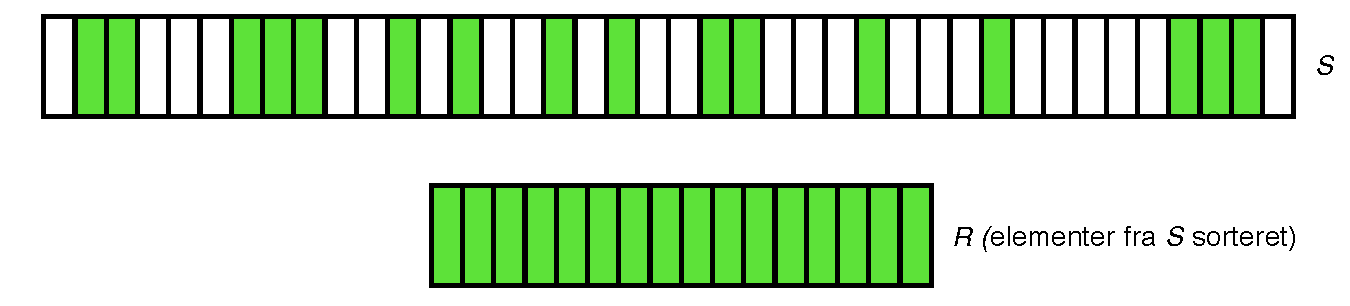
\includegraphics[width=\textwidth]{lazy1.pdf}
  \end{center}
  %\caption{Array $s$, hvor $n^{3/4}$ elementer er valgt og sorteret $R$}
  \label{fig:lazy1}
\end{figure}

Herefter fås $x = kn^{-1/4} \approx 15$ og herved $l = 8$ og $h = 16$. Derved må $a$, som er det 8'te mindste element i $R$ og $b$, som er det 16'te mindste element i $R$, kunne ses som:
\begin{figure}[H]
  \begin{center}
  
\includegraphics[width=\textwidth]{lazy2.pdf}
  \end{center}
  %\caption{$a$ og $b$ i sorteret $R$}
  \label{fig:lazy2}
\end{figure}

Herefter bestemmer vi rank af $a$ og $b$, $r_S(a)$ og $r_S(b)$, i forhold til den originale liste $S$. Samtidig laver vi ud fra dette vores nye liste $P$. Det er dette, som bidrager med vores $2n$ sammenligninger. Hvis vi tegner vores nye liste $P$, sammenholdt med $S$ hvor den var sorteret, kunne det se således ud:
\begin{figure}[H]
  \begin{center}
  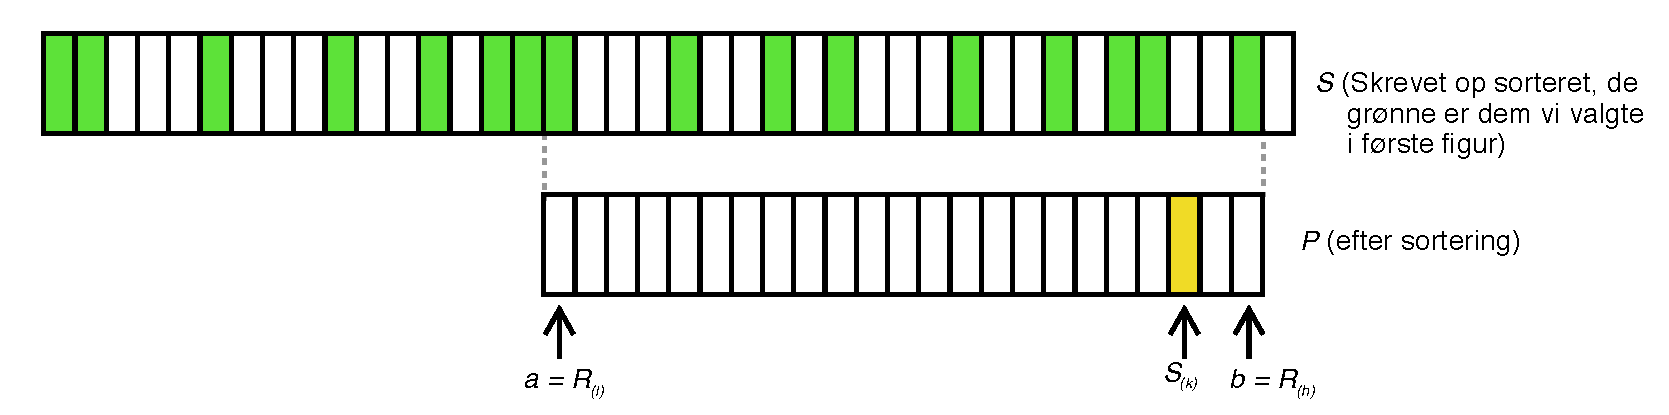
\includegraphics[width=\textwidth]{lazy3.pdf}
  \end{center}
  %\caption{caption}
  \label{fig:lazy3}
\end{figure}

Her svarer de markerede grønne felter til de 16 felter vi valgte tilfældigt i $S$ til at starte med, men nu hvor den (blot på figuren, ikke i algoritmen) er skrevet op sorteret for at kunne sammenligne med $P$, som bliver sorteret af algoritmen. Vi fandt her, at $r_S(a) = 17$ og $r_S(b) = 39$.\\

Da vi ikke fejler nogle af vores test i step 4 af algoritmen fortsætter vi til step 5. Vi får herved $P_{(k - r_S(a) + 1)} = P_{(37 - 17 + 1)} = P_{(21)}$, som svarer til $S_{(37)}$ hvilket netop var hvad vi skulle bestemme (markeret med gult på figuren).\\

På et større taleksempel ville det typisk relativt set være en mindre del af $R$ der ville blive valgt ud.



\subsection{Sandsynlighed for succes i første iteration}
Med sandsynlighed $1 - O(n^{-1/4})$ er der succes i første iteration af linje 4 og dermed laver algoritmen kun $2n + o(n)$ sammenligninger.\\

\textbf{Bevis}:\\
Vi har tre mulige fejltyper:\\
Fejltype 1: $S_{(k)} < a$\\
Fejltype 2: $S_{(k)} > b$\\
Fejltype 3: $|P| > 4 n^{3/4} + 2$.\\\\

Vi fokuserer på fejltype 1. Det er en fejl vi får i følgende tilfælde:
\begin{figure}[H]
  \begin{center}
  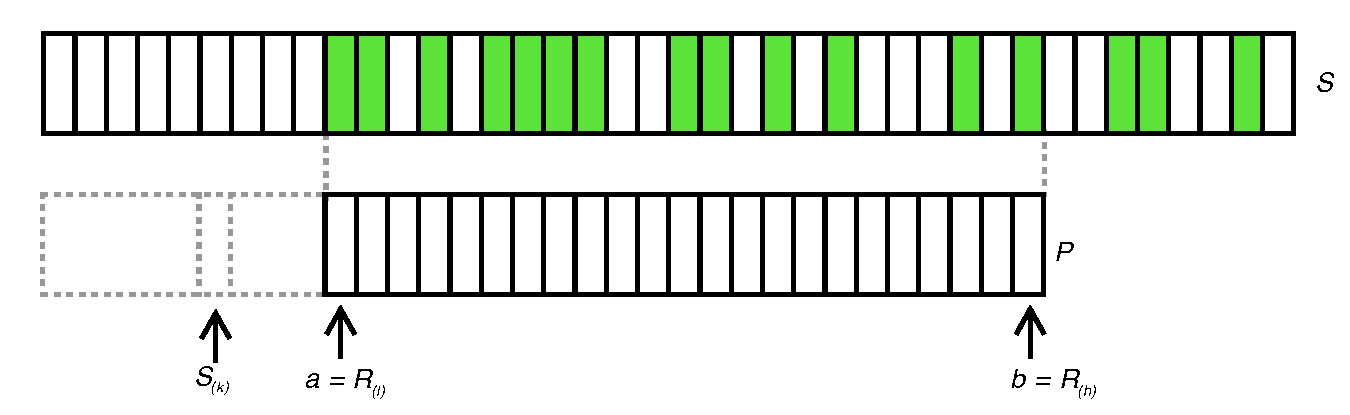
\includegraphics[width=\textwidth]{fejltype1.pdf}
  \end{center}
  %\caption{caption}
  \label{fig:fejltype1}
\end{figure}




For alle vores udtrukne elementer $i = 1, ..., n^{3/4}$, lad
$
X_i =
\begin{cases}
	1 & \text{hvis det $i$'te sample $\leq S_{(k)}$}\\
	0 & \text{ellers}
\end{cases}
$\\

Da er $\E[X_i] = \P{X_i = 1} = \frac{k}{n}$, som det tydeligt ses på figuren da de første $1, ..., k$ elementer naturligvis vil være $\leq k$, og der er $n$ elementer i alt.

Lad $X = \sum_{i=1}^{n^{3/4}} X_i$. Så får vi den forventede værdi til:
$$
\mu_X = \sum_{i=1}^{n^{3/4}} \mu_{X_i} = \sum_{i=1}^{n^{3/4}} \frac{k}{n} = n^{3/4} * \frac{k}{n} = kn^{-1/4} = x
$$

I eksemplet på fejltypen ovenfor er $X = 0$ og $l = 1$.

Og da kan vi beregne:
\begin{align}
  \P{S_{(k)} < a} &= \P{X < l} \label{eq:x-less-l}  \\
  &= \P{X < \max \left\{ \floor{x - \sqrt{n}}, 1 \right\} } \nonumber\\
  &\leq \P{X \leq \floor{x - \sqrt{n}}} \label{eq:fjern-max} \\
  &\leq \P{X \leq x - \sqrt{n}} \nonumber\\
  &= \P{X \leq \mu_X - \sqrt{n}} \label{eq:p-simpel}
\end{align}

I \cref{eq:x-less-l} bruger vi, at $X$ er antal elementer (i en sorteret udgave af $S$) før eller ved placeringen af $S_{(k)}$. $l$ bestemmer hvilket element vi starter ved af de udtrukne. Derfor må fejltype 1 opstå, når antallet af udtrukne elementer der opfylder at være $\leq S_{(k)}$ er et mindre antal end vores ''start-index'' for de udtrukne elementer, $l$.\\
I \cref{eq:fjern-max} benytter vi, at såfremt 1 er max, så kan $X$ stadig lavest være 0. Derfor må $\leq$ af det andet udtryk stadig gælde. Vores $\leq$ mellem linjerne får vi fra at vi nu siger $\leq$ inde i selve sandsynligheden.\\

Nu bruger vi det lemma, at givet \emph{uafhængige} stokastiske variable $Y_1, ..., Y_m$, hvor vi lader $Y = \sum_{i=1}^m Y_i$, da er variansen $\sigma_Y^2 = \sum_{i=1}^m {\sigma_{Y_i}}^2$:
\begin{align}
  \sigma_X^2 &= \sum_{i=1}^{n^{3/4}} {\sigma_{X_i}}^2 \nonumber \\
  &= \sum_{i=1}^{n^{3/4}} \frac{k}{n} \p{ 1 - \frac{k}{n} } \label{eq:faa-paren} \\
  &\leq \sum_{i=1}^{n^{3/4}} \frac{1}{4} \label{eq:paren-to-max} \\
  &= \frac{n^{3/4}}{4} \nonumber \\
  &\Updownarrow \nonumber \\
  \sigma_X &= \frac{n^{3/8}}{2} \label{eq:std-dev}
\end{align}

I \cref{eq:faa-paren} bruger vi at de stokastiske variable $X_i$ er Bernoulli trials som har variansen $\sigma_{X_i}^2 = p*(1-p)$ hvor $p = \P{X_i = 1} = k/n$.\\
I \cref{eq:paren-to-max} benytter vi, at udtrykket $p(1 - p)$ er størst når $p = 1/2$ og da bliver $1/4$.\\
I \cref{eq:std-dev} tager vi kvadratroden og får herved standardafvigelsen.

Regner vi nu videre på \cref{eq:p-simpel} med denne viden får vi:
\begin{align}
  \P{S_{(k)} < a} &\leq \P{X \leq \mu_X - \sqrt{n}} \nonumber \\
  &= \P{-X \geq -\mu_X + \sqrt{n}} \nonumber \\
  &= \P{\mu_X - X \geq \sqrt{n}} \nonumber \\
  &\leq \P{|\mu_X - X| \geq \sqrt{n}}  \nonumber \\
  &= \P{|\mu_X - X| \geq 2n^{1/8} * \frac{n^{3/8}}{2}  } \label{eq:skriv-smart} \\
  &\leq \P{ |\mu_X - X| \geq 2n^{1/8} \sigma_X } \label{eq:skriv-til-sigma} \\
  &\leq \frac{1}{\p{2n^{1/8}}^2} \label{eq:brug-chebyshev} \\
  &\leq \frac{1}{4n^{1/4}} \nonumber \\
  &= O(n^{-1/4}) \nonumber
\end{align}

I \cref{eq:skriv-smart} skriver vi blot $\sqrt{n} = n^{1/2}$ på en smart måde for at kunne bruge $\sigma_X$.\\
I \cref{eq:skriv-til-sigma} indsætter vi så blot vores $\sigma_X$.\\
I \cref{eq:brug-chebyshev} bruger vi Chebyshevs ulighed.\\

Herved har vi altså vist, at sandsynligheden for at en fejl af fejltype 1 opstår i første iteration af algoritmen kun er $O(n^{-1/4})$, og at den herved kun laver $2n + o(n)$ sammenligninger ($2n$ fra at bestemme rank af $a$ og $b$ og $o(n)$ fra sorteringen af $R$ og $P$).\\

Beviset for fejltype 2 er symmetrisk. Og fejltype 3 vil vi ikke beskæftige os med.
